% Options for packages loaded elsewhere
\PassOptionsToPackage{unicode}{hyperref}
\PassOptionsToPackage{hyphens}{url}
\PassOptionsToPackage{dvipsnames,svgnames,x11names}{xcolor}
%
\documentclass[
  letterpaper,
  DIV=11,
  numbers=noendperiod]{scrartcl}

\usepackage{amsmath,amssymb}
\usepackage{iftex}
\ifPDFTeX
  \usepackage[T1]{fontenc}
  \usepackage[utf8]{inputenc}
  \usepackage{textcomp} % provide euro and other symbols
\else % if luatex or xetex
  \usepackage{unicode-math}
  \defaultfontfeatures{Scale=MatchLowercase}
  \defaultfontfeatures[\rmfamily]{Ligatures=TeX,Scale=1}
\fi
\usepackage{lmodern}
\ifPDFTeX\else  
    % xetex/luatex font selection
\fi
% Use upquote if available, for straight quotes in verbatim environments
\IfFileExists{upquote.sty}{\usepackage{upquote}}{}
\IfFileExists{microtype.sty}{% use microtype if available
  \usepackage[]{microtype}
  \UseMicrotypeSet[protrusion]{basicmath} % disable protrusion for tt fonts
}{}
\makeatletter
\@ifundefined{KOMAClassName}{% if non-KOMA class
  \IfFileExists{parskip.sty}{%
    \usepackage{parskip}
  }{% else
    \setlength{\parindent}{0pt}
    \setlength{\parskip}{6pt plus 2pt minus 1pt}}
}{% if KOMA class
  \KOMAoptions{parskip=half}}
\makeatother
\usepackage{xcolor}
\setlength{\emergencystretch}{3em} % prevent overfull lines
\setcounter{secnumdepth}{-\maxdimen} % remove section numbering
% Make \paragraph and \subparagraph free-standing
\makeatletter
\ifx\paragraph\undefined\else
  \let\oldparagraph\paragraph
  \renewcommand{\paragraph}{
    \@ifstar
      \xxxParagraphStar
      \xxxParagraphNoStar
  }
  \newcommand{\xxxParagraphStar}[1]{\oldparagraph*{#1}\mbox{}}
  \newcommand{\xxxParagraphNoStar}[1]{\oldparagraph{#1}\mbox{}}
\fi
\ifx\subparagraph\undefined\else
  \let\oldsubparagraph\subparagraph
  \renewcommand{\subparagraph}{
    \@ifstar
      \xxxSubParagraphStar
      \xxxSubParagraphNoStar
  }
  \newcommand{\xxxSubParagraphStar}[1]{\oldsubparagraph*{#1}\mbox{}}
  \newcommand{\xxxSubParagraphNoStar}[1]{\oldsubparagraph{#1}\mbox{}}
\fi
\makeatother

\usepackage{color}
\usepackage{fancyvrb}
\newcommand{\VerbBar}{|}
\newcommand{\VERB}{\Verb[commandchars=\\\{\}]}
\DefineVerbatimEnvironment{Highlighting}{Verbatim}{commandchars=\\\{\}}
% Add ',fontsize=\small' for more characters per line
\usepackage{framed}
\definecolor{shadecolor}{RGB}{241,243,245}
\newenvironment{Shaded}{\begin{snugshade}}{\end{snugshade}}
\newcommand{\AlertTok}[1]{\textcolor[rgb]{0.68,0.00,0.00}{#1}}
\newcommand{\AnnotationTok}[1]{\textcolor[rgb]{0.37,0.37,0.37}{#1}}
\newcommand{\AttributeTok}[1]{\textcolor[rgb]{0.40,0.45,0.13}{#1}}
\newcommand{\BaseNTok}[1]{\textcolor[rgb]{0.68,0.00,0.00}{#1}}
\newcommand{\BuiltInTok}[1]{\textcolor[rgb]{0.00,0.23,0.31}{#1}}
\newcommand{\CharTok}[1]{\textcolor[rgb]{0.13,0.47,0.30}{#1}}
\newcommand{\CommentTok}[1]{\textcolor[rgb]{0.37,0.37,0.37}{#1}}
\newcommand{\CommentVarTok}[1]{\textcolor[rgb]{0.37,0.37,0.37}{\textit{#1}}}
\newcommand{\ConstantTok}[1]{\textcolor[rgb]{0.56,0.35,0.01}{#1}}
\newcommand{\ControlFlowTok}[1]{\textcolor[rgb]{0.00,0.23,0.31}{\textbf{#1}}}
\newcommand{\DataTypeTok}[1]{\textcolor[rgb]{0.68,0.00,0.00}{#1}}
\newcommand{\DecValTok}[1]{\textcolor[rgb]{0.68,0.00,0.00}{#1}}
\newcommand{\DocumentationTok}[1]{\textcolor[rgb]{0.37,0.37,0.37}{\textit{#1}}}
\newcommand{\ErrorTok}[1]{\textcolor[rgb]{0.68,0.00,0.00}{#1}}
\newcommand{\ExtensionTok}[1]{\textcolor[rgb]{0.00,0.23,0.31}{#1}}
\newcommand{\FloatTok}[1]{\textcolor[rgb]{0.68,0.00,0.00}{#1}}
\newcommand{\FunctionTok}[1]{\textcolor[rgb]{0.28,0.35,0.67}{#1}}
\newcommand{\ImportTok}[1]{\textcolor[rgb]{0.00,0.46,0.62}{#1}}
\newcommand{\InformationTok}[1]{\textcolor[rgb]{0.37,0.37,0.37}{#1}}
\newcommand{\KeywordTok}[1]{\textcolor[rgb]{0.00,0.23,0.31}{\textbf{#1}}}
\newcommand{\NormalTok}[1]{\textcolor[rgb]{0.00,0.23,0.31}{#1}}
\newcommand{\OperatorTok}[1]{\textcolor[rgb]{0.37,0.37,0.37}{#1}}
\newcommand{\OtherTok}[1]{\textcolor[rgb]{0.00,0.23,0.31}{#1}}
\newcommand{\PreprocessorTok}[1]{\textcolor[rgb]{0.68,0.00,0.00}{#1}}
\newcommand{\RegionMarkerTok}[1]{\textcolor[rgb]{0.00,0.23,0.31}{#1}}
\newcommand{\SpecialCharTok}[1]{\textcolor[rgb]{0.37,0.37,0.37}{#1}}
\newcommand{\SpecialStringTok}[1]{\textcolor[rgb]{0.13,0.47,0.30}{#1}}
\newcommand{\StringTok}[1]{\textcolor[rgb]{0.13,0.47,0.30}{#1}}
\newcommand{\VariableTok}[1]{\textcolor[rgb]{0.07,0.07,0.07}{#1}}
\newcommand{\VerbatimStringTok}[1]{\textcolor[rgb]{0.13,0.47,0.30}{#1}}
\newcommand{\WarningTok}[1]{\textcolor[rgb]{0.37,0.37,0.37}{\textit{#1}}}

\providecommand{\tightlist}{%
  \setlength{\itemsep}{0pt}\setlength{\parskip}{0pt}}\usepackage{longtable,booktabs,array}
\usepackage{calc} % for calculating minipage widths
% Correct order of tables after \paragraph or \subparagraph
\usepackage{etoolbox}
\makeatletter
\patchcmd\longtable{\par}{\if@noskipsec\mbox{}\fi\par}{}{}
\makeatother
% Allow footnotes in longtable head/foot
\IfFileExists{footnotehyper.sty}{\usepackage{footnotehyper}}{\usepackage{footnote}}
\makesavenoteenv{longtable}
\usepackage{graphicx}
\makeatletter
\newsavebox\pandoc@box
\newcommand*\pandocbounded[1]{% scales image to fit in text height/width
  \sbox\pandoc@box{#1}%
  \Gscale@div\@tempa{\textheight}{\dimexpr\ht\pandoc@box+\dp\pandoc@box\relax}%
  \Gscale@div\@tempb{\linewidth}{\wd\pandoc@box}%
  \ifdim\@tempb\p@<\@tempa\p@\let\@tempa\@tempb\fi% select the smaller of both
  \ifdim\@tempa\p@<\p@\scalebox{\@tempa}{\usebox\pandoc@box}%
  \else\usebox{\pandoc@box}%
  \fi%
}
% Set default figure placement to htbp
\def\fps@figure{htbp}
\makeatother

\KOMAoption{captions}{tableheading}
\makeatletter
\@ifpackageloaded{caption}{}{\usepackage{caption}}
\AtBeginDocument{%
\ifdefined\contentsname
  \renewcommand*\contentsname{Table of contents}
\else
  \newcommand\contentsname{Table of contents}
\fi
\ifdefined\listfigurename
  \renewcommand*\listfigurename{List of Figures}
\else
  \newcommand\listfigurename{List of Figures}
\fi
\ifdefined\listtablename
  \renewcommand*\listtablename{List of Tables}
\else
  \newcommand\listtablename{List of Tables}
\fi
\ifdefined\figurename
  \renewcommand*\figurename{Figure}
\else
  \newcommand\figurename{Figure}
\fi
\ifdefined\tablename
  \renewcommand*\tablename{Table}
\else
  \newcommand\tablename{Table}
\fi
}
\@ifpackageloaded{float}{}{\usepackage{float}}
\floatstyle{ruled}
\@ifundefined{c@chapter}{\newfloat{codelisting}{h}{lop}}{\newfloat{codelisting}{h}{lop}[chapter]}
\floatname{codelisting}{Listing}
\newcommand*\listoflistings{\listof{codelisting}{List of Listings}}
\makeatother
\makeatletter
\makeatother
\makeatletter
\@ifpackageloaded{caption}{}{\usepackage{caption}}
\@ifpackageloaded{subcaption}{}{\usepackage{subcaption}}
\makeatother

\usepackage{bookmark}

\IfFileExists{xurl.sty}{\usepackage{xurl}}{} % add URL line breaks if available
\urlstyle{same} % disable monospaced font for URLs
\hypersetup{
  pdftitle={Basic Statistics},
  colorlinks=true,
  linkcolor={blue},
  filecolor={Maroon},
  citecolor={Blue},
  urlcolor={Blue},
  pdfcreator={LaTeX via pandoc}}


\title{Basic Statistics}
\author{}
\date{}

\begin{document}
\maketitle


\subsection{Introduction}\label{introduction}

In this small document we will practice basic statistics. We will
explore the dataset \texttt{mtcars}, which is included in the basic R
installation.

\subsection{Libraries and Data}\label{libraries-and-data}

We will begin by loading the libraries we will use. Instead of loading
our libraries one at a time, we can just load \texttt{tidyverse}, which
includes all the tools that we'll need

\begin{Shaded}
\begin{Highlighting}[]
\FunctionTok{library}\NormalTok{(summarytools)}
\FunctionTok{library}\NormalTok{(tidyverse)}
\end{Highlighting}
\end{Shaded}

\begin{verbatim}
-- Attaching core tidyverse packages ------------------------ tidyverse 2.0.0 --
v dplyr     1.1.4     v readr     2.1.5
v forcats   1.0.0     v stringr   1.5.1
v ggplot2   3.5.2     v tibble    3.3.0
v lubridate 1.9.4     v tidyr     1.3.1
v purrr     1.1.0     
-- Conflicts ------------------------------------------ tidyverse_conflicts() --
x dplyr::filter() masks stats::filter()
x dplyr::lag()    masks stats::lag()
x tibble::view()  masks summarytools::view()
i Use the conflicted package (<http://conflicted.r-lib.org/>) to force all conflicts to become errors
\end{verbatim}

Now, we load our dataset

\begin{Shaded}
\begin{Highlighting}[]
\FunctionTok{attach}\NormalTok{(mtcars)}
\end{Highlighting}
\end{Shaded}

\begin{verbatim}
The following object is masked from package:ggplot2:

    mpg
\end{verbatim}

\subsection{Exploring the dataset}\label{exploring-the-dataset}

We can explore the contents of the dataset just by typing in its name

\begin{Shaded}
\begin{Highlighting}[]
\NormalTok{mtcars}
\end{Highlighting}
\end{Shaded}

\begin{verbatim}
                     mpg cyl  disp  hp drat    wt  qsec vs am gear carb
Mazda RX4           21.0   6 160.0 110 3.90 2.620 16.46  0  1    4    4
Mazda RX4 Wag       21.0   6 160.0 110 3.90 2.875 17.02  0  1    4    4
Datsun 710          22.8   4 108.0  93 3.85 2.320 18.61  1  1    4    1
Hornet 4 Drive      21.4   6 258.0 110 3.08 3.215 19.44  1  0    3    1
Hornet Sportabout   18.7   8 360.0 175 3.15 3.440 17.02  0  0    3    2
Valiant             18.1   6 225.0 105 2.76 3.460 20.22  1  0    3    1
Duster 360          14.3   8 360.0 245 3.21 3.570 15.84  0  0    3    4
Merc 240D           24.4   4 146.7  62 3.69 3.190 20.00  1  0    4    2
Merc 230            22.8   4 140.8  95 3.92 3.150 22.90  1  0    4    2
Merc 280            19.2   6 167.6 123 3.92 3.440 18.30  1  0    4    4
Merc 280C           17.8   6 167.6 123 3.92 3.440 18.90  1  0    4    4
Merc 450SE          16.4   8 275.8 180 3.07 4.070 17.40  0  0    3    3
Merc 450SL          17.3   8 275.8 180 3.07 3.730 17.60  0  0    3    3
Merc 450SLC         15.2   8 275.8 180 3.07 3.780 18.00  0  0    3    3
Cadillac Fleetwood  10.4   8 472.0 205 2.93 5.250 17.98  0  0    3    4
Lincoln Continental 10.4   8 460.0 215 3.00 5.424 17.82  0  0    3    4
Chrysler Imperial   14.7   8 440.0 230 3.23 5.345 17.42  0  0    3    4
Fiat 128            32.4   4  78.7  66 4.08 2.200 19.47  1  1    4    1
Honda Civic         30.4   4  75.7  52 4.93 1.615 18.52  1  1    4    2
Toyota Corolla      33.9   4  71.1  65 4.22 1.835 19.90  1  1    4    1
Toyota Corona       21.5   4 120.1  97 3.70 2.465 20.01  1  0    3    1
Dodge Challenger    15.5   8 318.0 150 2.76 3.520 16.87  0  0    3    2
AMC Javelin         15.2   8 304.0 150 3.15 3.435 17.30  0  0    3    2
Camaro Z28          13.3   8 350.0 245 3.73 3.840 15.41  0  0    3    4
Pontiac Firebird    19.2   8 400.0 175 3.08 3.845 17.05  0  0    3    2
Fiat X1-9           27.3   4  79.0  66 4.08 1.935 18.90  1  1    4    1
Porsche 914-2       26.0   4 120.3  91 4.43 2.140 16.70  0  1    5    2
Lotus Europa        30.4   4  95.1 113 3.77 1.513 16.90  1  1    5    2
Ford Pantera L      15.8   8 351.0 264 4.22 3.170 14.50  0  1    5    4
Ferrari Dino        19.7   6 145.0 175 3.62 2.770 15.50  0  1    5    6
Maserati Bora       15.0   8 301.0 335 3.54 3.570 14.60  0  1    5    8
Volvo 142E          21.4   4 121.0 109 4.11 2.780 18.60  1  1    4    2
\end{verbatim}

The dataset consists of 11 variables for 32 records. Let's explore the
variable \texttt{mpg} by first creating a new variable:

\begin{Shaded}
\begin{Highlighting}[]
\NormalTok{mtcars\_mpg }\OtherTok{\textless{}{-}}\NormalTok{ mtcars}\SpecialCharTok{$}\NormalTok{mpg}
\end{Highlighting}
\end{Shaded}

\subsection{Descriptive statistics}\label{descriptive-statistics}

\subsubsection{Minimum and maximum}\label{minimum-and-maximum}

Minimum and maximum can be found thanks to the \texttt{min()} and
\texttt{max()} functions:

\begin{Shaded}
\begin{Highlighting}[]
\FunctionTok{min}\NormalTok{(mtcars\_mpg)}
\end{Highlighting}
\end{Shaded}

\begin{verbatim}
[1] 10.4
\end{verbatim}

\begin{Shaded}
\begin{Highlighting}[]
\FunctionTok{max}\NormalTok{(mtcars\_mpg)}
\end{Highlighting}
\end{Shaded}

\begin{verbatim}
[1] 33.9
\end{verbatim}

Alternatively the \texttt{range()} function gives you the minimum and
maximum directly:

\begin{Shaded}
\begin{Highlighting}[]
\NormalTok{rng }\OtherTok{\textless{}{-}} \FunctionTok{range}\NormalTok{(mtcars\_mpg)}
\NormalTok{rng}
\end{Highlighting}
\end{Shaded}

\begin{verbatim}
[1] 10.4 33.9
\end{verbatim}

Note that the output of the \texttt{range()} function is actually an
object containing the minimum and maximum (in that order). This means
you can actually access the minimum with

\begin{Shaded}
\begin{Highlighting}[]
\NormalTok{rng[}\DecValTok{1}\NormalTok{]}
\end{Highlighting}
\end{Shaded}

\begin{verbatim}
[1] 10.4
\end{verbatim}

\begin{Shaded}
\begin{Highlighting}[]
\NormalTok{rng[}\DecValTok{2}\NormalTok{]}
\end{Highlighting}
\end{Shaded}

\begin{verbatim}
[1] 33.9
\end{verbatim}

This reminds us that, in R, there are often several ways to arrive at
the same result. The method that uses the shortest piece of code is
usually preferred as a shorter piece of code is less prone to coding
errors and more readable.

\subsubsection{Measures of central
tendency}\label{measures-of-central-tendency}

\paragraph{Mean}\label{mean}

The mean can be computed with the \texttt{mean()} function

\begin{Shaded}
\begin{Highlighting}[]
\FunctionTok{mean}\NormalTok{(mtcars\_mpg)}
\end{Highlighting}
\end{Shaded}

\begin{verbatim}
[1] 20.09062
\end{verbatim}

\emph{Tips:}

\begin{itemize}
\item
  if there is at least one missing value in your dataset, use
  \texttt{mean(data,\ na.rm\ =\ TRUE)} to compute the mean with the NA
  excluded. This argument can be used for many other functions, not only
  the mean
\item
  for a truncated mean, use \texttt{mean(data,\ trim\ =\ 0.10)} and
  change the \texttt{trim} argument to your needs
\end{itemize}

\paragraph{Median}\label{median}

The median can be computed thanks to the \texttt{median()} function:

\begin{Shaded}
\begin{Highlighting}[]
\FunctionTok{median}\NormalTok{(mtcars\_mpg)}
\end{Highlighting}
\end{Shaded}

\begin{verbatim}
[1] 19.2
\end{verbatim}

or with the \texttt{quantile()} function:

\begin{Shaded}
\begin{Highlighting}[]
\FunctionTok{quantile}\NormalTok{(mtcars\_mpg, }\FloatTok{0.5}\NormalTok{)}
\end{Highlighting}
\end{Shaded}

\begin{verbatim}
 50% 
19.2 
\end{verbatim}

since the quantile of order 0.5 corresponds to the median.

\paragraph{Quantiles}\label{quantiles}

Remember that the \(q\) quantile, with \(0\le q\le 1\), corresponds to
the data point below which we have a fraction \(q\) of the data points
when sorted in ascending order. So, for instance, the median corresponds
to the \(0.5\) quantile because 50\% of the sorted data is below it.

Other important quantiles are the 0.25 and 0.75 quantiles, also called
the 1st and the 3rd quartiles. They can be obtained using the
\texttt{quantile()} function

\begin{Shaded}
\begin{Highlighting}[]
\FunctionTok{quantile}\NormalTok{(mtcars\_mpg, }\FloatTok{0.25}\NormalTok{) }\CommentTok{\# first quartile}
\end{Highlighting}
\end{Shaded}

\begin{verbatim}
   25% 
15.425 
\end{verbatim}

\begin{Shaded}
\begin{Highlighting}[]
\FunctionTok{quantile}\NormalTok{(mtcars\_mpg, }\FloatTok{0.75}\NormalTok{) }\CommentTok{\# third quartile}
\end{Highlighting}
\end{Shaded}

\begin{verbatim}
 75% 
22.8 
\end{verbatim}

\paragraph{Mode}\label{mode}

The mode is the value that has highest number of occurrences in a set of
data. Unike mean and median, mode can have both numeric and character
data.

R does not have a standard in-built function to calculate mode. So we
create a user function to calculate mode of a data set in R. This
function takes the vector as input and gives the mode value as output.

\begin{Shaded}
\begin{Highlighting}[]
\NormalTok{getmode }\OtherTok{\textless{}{-}} \ControlFlowTok{function}\NormalTok{(v) \{}
\NormalTok{   uniqv }\OtherTok{\textless{}{-}} \FunctionTok{unique}\NormalTok{(v)}
\NormalTok{   uniqv[}\FunctionTok{which.max}\NormalTok{(}\FunctionTok{tabulate}\NormalTok{(}\FunctionTok{match}\NormalTok{(v, uniqv)))]}
\NormalTok{\}}

\FunctionTok{getmode}\NormalTok{(mtcars\_mpg)}
\end{Highlighting}
\end{Shaded}

\begin{verbatim}
[1] 21
\end{verbatim}

\subsubsection{Measures of variation}\label{measures-of-variation}

\subsubsection{Range}\label{range}

The range of the data can be easily computed by subtracting the minimum
from the maximum

\begin{Shaded}
\begin{Highlighting}[]
\NormalTok{rng[}\DecValTok{2}\NormalTok{]}\SpecialCharTok{{-}}\NormalTok{rng[}\DecValTok{1}\NormalTok{]}
\end{Highlighting}
\end{Shaded}

\begin{verbatim}
[1] 23.5
\end{verbatim}

\paragraph{Interquartile range}\label{interquartile-range}

The interquartile range (i.e., the difference between the first and
third quartiles) can be computed with the \texttt{IQR()} function

\begin{Shaded}
\begin{Highlighting}[]
\FunctionTok{IQR}\NormalTok{(mtcars\_mpg)}
\end{Highlighting}
\end{Shaded}

\begin{verbatim}
[1] 7.375
\end{verbatim}

\paragraph{Standard deviation and
variance}\label{standard-deviation-and-variance}

The standard deviation and the variance are computed with the
\texttt{sd()} and \texttt{var()} functions, respectively. These
functions correspond to the sample standard deviation and variance,
since R assumes that the data corresponds to a sample of the population.

\begin{Shaded}
\begin{Highlighting}[]
\FunctionTok{sd}\NormalTok{(mtcars\_mpg)}
\end{Highlighting}
\end{Shaded}

\begin{verbatim}
[1] 6.026948
\end{verbatim}

\begin{Shaded}
\begin{Highlighting}[]
\FunctionTok{var}\NormalTok{(mtcars\_mpg)}
\end{Highlighting}
\end{Shaded}

\begin{verbatim}
[1] 36.3241
\end{verbatim}

It is easy to see that the variance is the square of the standar
deviation, as it should be.

\begin{Shaded}
\begin{Highlighting}[]
\FunctionTok{var}\NormalTok{(mtcars\_mpg) }\SpecialCharTok{==}\NormalTok{ (}\FunctionTok{sd}\NormalTok{(mtcars\_mpg))}\SpecialCharTok{\^{}}\DecValTok{2}
\end{Highlighting}
\end{Shaded}

\begin{verbatim}
[1] TRUE
\end{verbatim}

\subsubsection{Descriptive statistics of several variables at a
time}\label{descriptive-statistics-of-several-variables-at-a-time}

We can use the \texttt{lapply()} function to calculate a statistic of
several variables at a time. For instance, if we wanted to find the mean
of all numerical variables in our data set, we would type

\begin{Shaded}
\begin{Highlighting}[]
\FunctionTok{lapply}\NormalTok{(mtcars,mean)}
\end{Highlighting}
\end{Shaded}

\begin{verbatim}
$mpg
[1] 20.09062

$cyl
[1] 6.1875

$disp
[1] 230.7219

$hp
[1] 146.6875

$drat
[1] 3.596563

$wt
[1] 3.21725

$qsec
[1] 17.84875

$vs
[1] 0.4375

$am
[1] 0.40625

$gear
[1] 3.6875

$carb
[1] 2.8125
\end{verbatim}

Better yet, in basic R we can use \texttt{summary()} to display all
relevant statistics of all numerical values in the dataset.

\begin{Shaded}
\begin{Highlighting}[]
\FunctionTok{summary}\NormalTok{(mtcars)}
\end{Highlighting}
\end{Shaded}

\begin{verbatim}
      mpg             cyl             disp             hp       
 Min.   :10.40   Min.   :4.000   Min.   : 71.1   Min.   : 52.0  
 1st Qu.:15.43   1st Qu.:4.000   1st Qu.:120.8   1st Qu.: 96.5  
 Median :19.20   Median :6.000   Median :196.3   Median :123.0  
 Mean   :20.09   Mean   :6.188   Mean   :230.7   Mean   :146.7  
 3rd Qu.:22.80   3rd Qu.:8.000   3rd Qu.:326.0   3rd Qu.:180.0  
 Max.   :33.90   Max.   :8.000   Max.   :472.0   Max.   :335.0  
      drat             wt             qsec             vs        
 Min.   :2.760   Min.   :1.513   Min.   :14.50   Min.   :0.0000  
 1st Qu.:3.080   1st Qu.:2.581   1st Qu.:16.89   1st Qu.:0.0000  
 Median :3.695   Median :3.325   Median :17.71   Median :0.0000  
 Mean   :3.597   Mean   :3.217   Mean   :17.85   Mean   :0.4375  
 3rd Qu.:3.920   3rd Qu.:3.610   3rd Qu.:18.90   3rd Qu.:1.0000  
 Max.   :4.930   Max.   :5.424   Max.   :22.90   Max.   :1.0000  
       am              gear            carb      
 Min.   :0.0000   Min.   :3.000   Min.   :1.000  
 1st Qu.:0.0000   1st Qu.:3.000   1st Qu.:2.000  
 Median :0.0000   Median :4.000   Median :2.000  
 Mean   :0.4062   Mean   :3.688   Mean   :2.812  
 3rd Qu.:1.0000   3rd Qu.:4.000   3rd Qu.:4.000  
 Max.   :1.0000   Max.   :5.000   Max.   :8.000  
\end{verbatim}

And even better with the \texttt{descr()} function from the
\texttt{summarytools} package:

\begin{Shaded}
\begin{Highlighting}[]
\FunctionTok{descr}\NormalTok{(mtcars)}
\end{Highlighting}
\end{Shaded}

\begin{verbatim}
Descriptive Statistics  
mtcars  
N: 32  

                        am     carb      cyl     disp     drat     gear       hp      mpg     qsec
----------------- -------- -------- -------- -------- -------- -------- -------- -------- --------
             Mean     0.41     2.81     6.19   230.72     3.60     3.69   146.69    20.09    17.85
          Std.Dev     0.50     1.62     1.79   123.94     0.53     0.74    68.56     6.03     1.79
              Min     0.00     1.00     4.00    71.10     2.76     3.00    52.00    10.40    14.50
               Q1     0.00     2.00     4.00   120.65     3.08     3.00    96.00    15.35    16.88
           Median     0.00     2.00     6.00   196.30     3.70     4.00   123.00    19.20    17.71
               Q3     1.00     4.00     8.00   334.00     3.92     4.00   180.00    22.80    18.90
              Max     1.00     8.00     8.00   472.00     4.93     5.00   335.00    33.90    22.90
              MAD     0.00     1.48     2.97   140.48     0.70     1.48    77.10     5.41     1.42
              IQR     1.00     2.00     4.00   205.18     0.84     1.00    83.50     7.38     2.01
               CV     1.23     0.57     0.29     0.54     0.15     0.20     0.47     0.30     0.10
         Skewness     0.36     1.05    -0.17     0.38     0.27     0.53     0.73     0.61     0.37
      SE.Skewness     0.41     0.41     0.41     0.41     0.41     0.41     0.41     0.41     0.41
         Kurtosis    -1.92     1.26    -1.76    -1.21    -0.71    -1.07    -0.14    -0.37     0.34
          N.Valid    32.00    32.00    32.00    32.00    32.00    32.00    32.00    32.00    32.00
                N    32.00    32.00    32.00    32.00    32.00    32.00    32.00    32.00    32.00
        Pct.Valid   100.00   100.00   100.00   100.00   100.00   100.00   100.00   100.00   100.00

Table: Table continues below

 

                        vs       wt
----------------- -------- --------
             Mean     0.44     3.22
          Std.Dev     0.50     0.98
              Min     0.00     1.51
               Q1     0.00     2.54
           Median     0.00     3.33
               Q3     1.00     3.65
              Max     1.00     5.42
              MAD     0.00     0.77
              IQR     1.00     1.03
               CV     1.15     0.30
         Skewness     0.24     0.42
      SE.Skewness     0.41     0.41
         Kurtosis    -2.00    -0.02
          N.Valid    32.00    32.00
                N    32.00    32.00
        Pct.Valid   100.00   100.00
\end{verbatim}

\subsection{Graphical analysis}\label{graphical-analysis}

Now that we have a numerical description of our dataset, we can proceed
to visualize this information. We will show how to get histograms,
boxplots, and other visualizations.

\subsubsection{Histogram}\label{histogram}

A histogram gives an idea about the distribution of a quantitative
variable. The idea is to break the range of values into intervals and
count how many observations fall into each interval. Histograms are a
bit similar to barplots, but histograms are used for quantitative
variables whereas barplots are used for qualitative variables. To draw a
histogram in R, use \texttt{hist()}:

\begin{Shaded}
\begin{Highlighting}[]
\FunctionTok{hist}\NormalTok{(mtcars\_mpg)}
\end{Highlighting}
\end{Shaded}

\pandocbounded{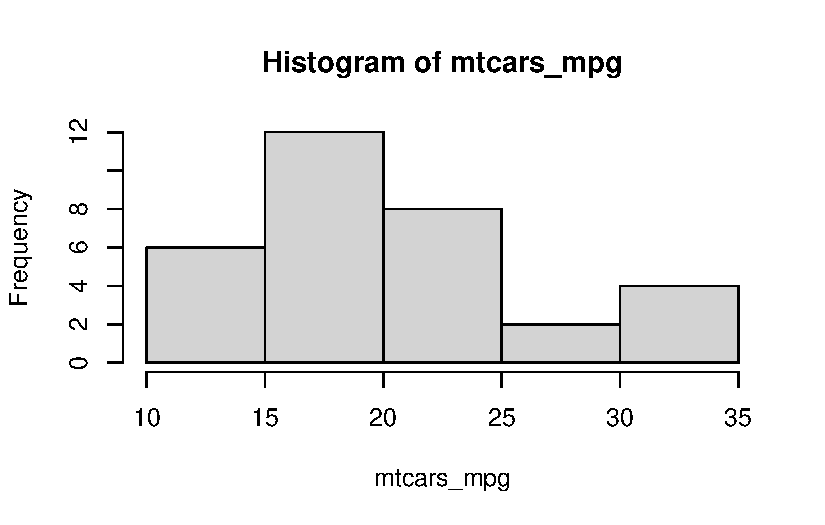
\includegraphics[keepaspectratio]{Descriptive_statistics_in_R_files/figure-pdf/unnamed-chunk-21-1.pdf}}

Add the arguments \texttt{breaks\ =} inside the \texttt{hist()} function
if you want to change the number of bins. A rule of thumb (known as
Sturges' law) is that the number of bins should be the rounded value of
the square root of the number of observations. The dataset includes 32
observations so in this case the number of bins can be set to 6.

\begin{Shaded}
\begin{Highlighting}[]
\FunctionTok{hist}\NormalTok{(mtcars\_mpg, }\AttributeTok{breaks=}\DecValTok{6}\NormalTok{)}
\end{Highlighting}
\end{Shaded}

\pandocbounded{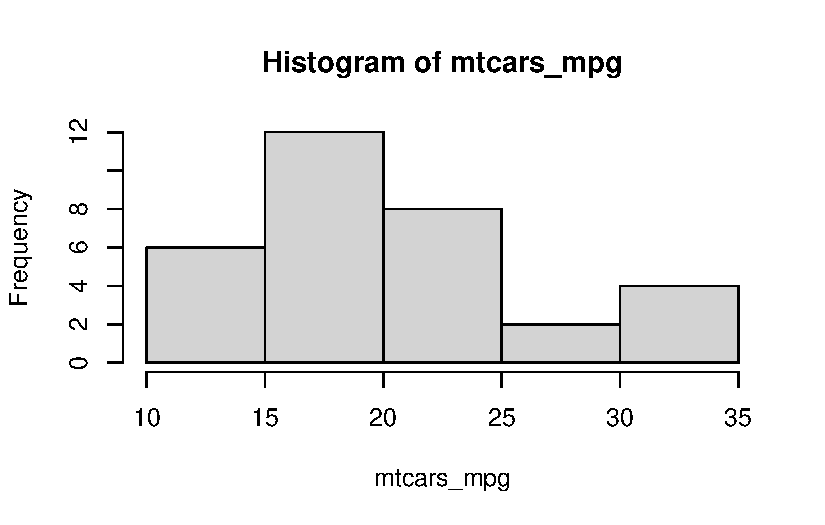
\includegraphics[keepaspectratio]{Descriptive_statistics_in_R_files/figure-pdf/unnamed-chunk-22-1.pdf}}

We can also use the \texttt{ggplot2} library, which is loaded by
\texttt{tidyverse} , to get a more customizable and visually appealing
histogram. A \texttt{ggplot} visualization is constructed in steps,
using a specialized grammar: we need the data, an aesthetics mapping,
and a geometry option, plus other customization options, in order to
construct the graph. The use of this grammar of graphics allows us to
construct different visualizations for the same dataset just by changing
one or more aspects of the graph.

For starters, we create a generic visualization for the dataset
\texttt{mtcars} :

\begin{Shaded}
\begin{Highlighting}[]
\NormalTok{cars\_graph }\OtherTok{\textless{}{-}} \FunctionTok{ggplot}\NormalTok{(mtcars)}
\end{Highlighting}
\end{Shaded}

Next, we add an aesthetics mapping for the \texttt{mpg} variable:

\begin{Shaded}
\begin{Highlighting}[]
\NormalTok{cars\_graph }\SpecialCharTok{+} \FunctionTok{aes}\NormalTok{(mpg)}
\end{Highlighting}
\end{Shaded}

\pandocbounded{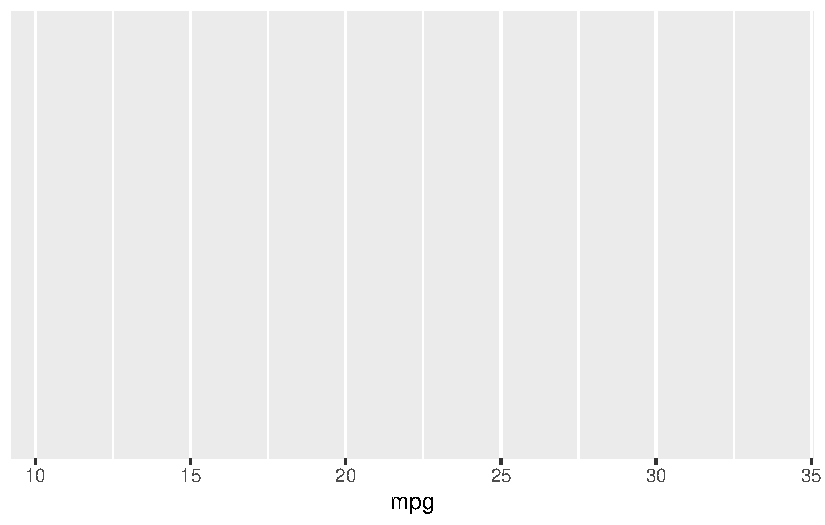
\includegraphics[keepaspectratio]{Descriptive_statistics_in_R_files/figure-pdf/unnamed-chunk-24-1.pdf}}

We get an empty canvas over which we can put any geometry we desire.
Even though we can add an aesthetics mapping after creating the
\texttt{ggplot} object, it is customary to create the object and the
aesthetics mapping together, and then add a geometry and other option.

\begin{Shaded}
\begin{Highlighting}[]
\NormalTok{cars\_graph }\OtherTok{\textless{}{-}} \FunctionTok{ggplot}\NormalTok{(mtcars, }\FunctionTok{aes}\NormalTok{(mpg))}
\end{Highlighting}
\end{Shaded}

For a basic histogram, we use \texttt{geom\_histogram()} .

\begin{Shaded}
\begin{Highlighting}[]
\NormalTok{cars\_graph }\SpecialCharTok{+} 
  \FunctionTok{geom\_histogram}\NormalTok{()}
\end{Highlighting}
\end{Shaded}

\begin{verbatim}
`stat_bin()` using `bins = 30`. Pick better value with `binwidth`.
\end{verbatim}

\pandocbounded{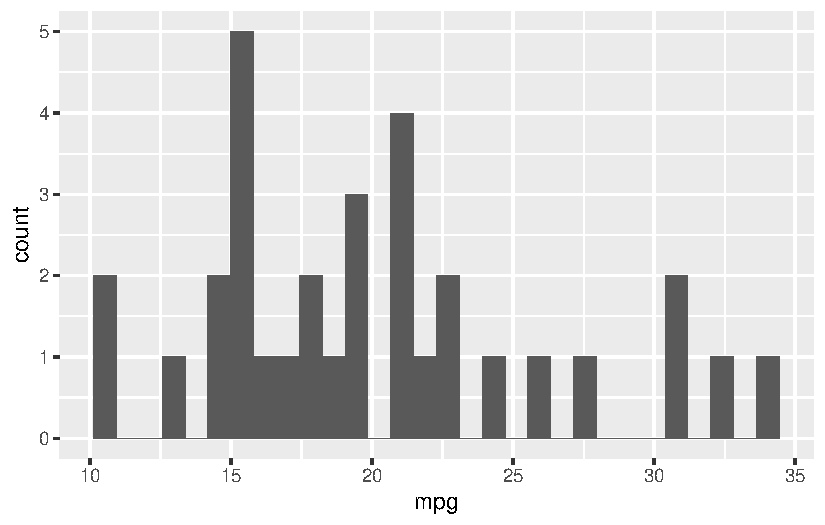
\includegraphics[keepaspectratio]{Descriptive_statistics_in_R_files/figure-pdf/unnamed-chunk-26-1.pdf}}

By default, the number of bins is 30. You can change this value with
\texttt{geom\_histogram(bins\ =\ 6)} for instance.

\begin{Shaded}
\begin{Highlighting}[]
\NormalTok{cars\_graph }\SpecialCharTok{+} 
  \FunctionTok{geom\_histogram}\NormalTok{(}\AttributeTok{bins =} \DecValTok{6}\NormalTok{)}
\end{Highlighting}
\end{Shaded}

\pandocbounded{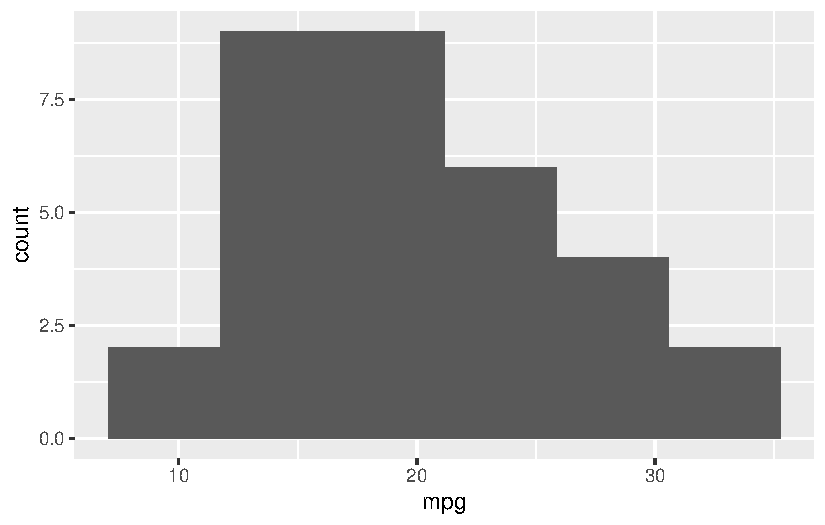
\includegraphics[keepaspectratio]{Descriptive_statistics_in_R_files/figure-pdf/unnamed-chunk-27-1.pdf}}

We can draw the distribution shape on top of the histogram, plus some
options to beautify the plot.

\begin{Shaded}
\begin{Highlighting}[]
\NormalTok{cars\_graph }\SpecialCharTok{+} 
  \FunctionTok{geom\_histogram}\NormalTok{(}\FunctionTok{aes}\NormalTok{(}\AttributeTok{y=}\FunctionTok{after\_stat}\NormalTok{(density)),}\AttributeTok{bins =} \DecValTok{6}\NormalTok{,}\AttributeTok{color =} \DecValTok{1}\NormalTok{, }\AttributeTok{fill =} \StringTok{"white"}\NormalTok{) }\SpecialCharTok{+}
  \FunctionTok{geom\_density}\NormalTok{(}\AttributeTok{alpha =} \FloatTok{0.25}\NormalTok{,}\AttributeTok{lwd =} \DecValTok{1}\NormalTok{, }\AttributeTok{colour =} \DecValTok{4}\NormalTok{,}
               \AttributeTok{fill =} \DecValTok{4}\NormalTok{) }\SpecialCharTok{+}
  \FunctionTok{labs}\NormalTok{(}\AttributeTok{title =} \StringTok{"Miles per gallon density plot and histogram"}\NormalTok{,}
       \AttributeTok{x =} \StringTok{"Miles per gallon"}\NormalTok{,}
       \AttributeTok{y =} \StringTok{"Density"}\NormalTok{)}
\end{Highlighting}
\end{Shaded}

\pandocbounded{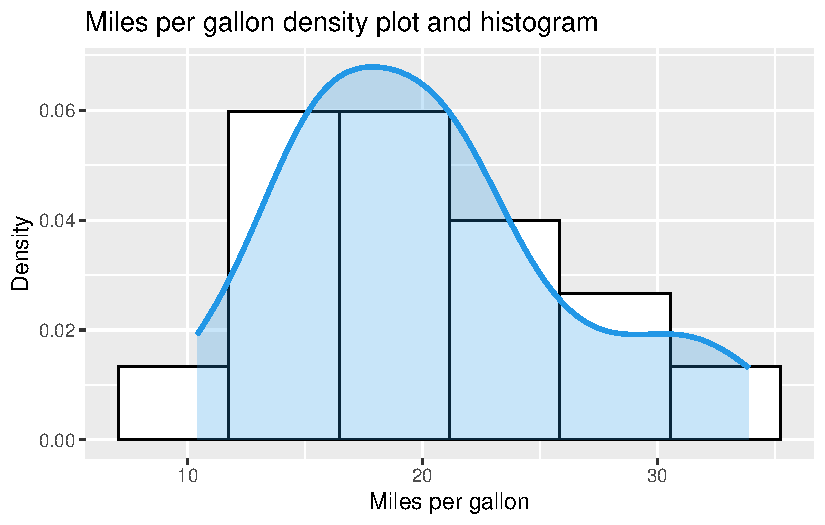
\includegraphics[keepaspectratio]{Descriptive_statistics_in_R_files/figure-pdf/unnamed-chunk-28-1.pdf}}

\subsubsection{Boxplots}\label{boxplots}

Boxplots are really useful in descriptive statistics and are often
underused (mostly because it is not well understood by the public). A
boxplot graphically represents the distribution of a quantitative
variable by visually displaying five common location summary (minimum,
median, first/third quartiles and maximum) and any observation that was
classified as a suspected
\href{http://localhost:6653/blog/outliers-detection-in-r/}{outlier}
using the interquartile range (IQR) criterion.

The IQR criterion means that all observations above
\(q_{0.75}+1.5\cdot IQR\) or below \(q_{0.25}-1.5\cdot IQR\) (where
\(q_{0.25}\) and \(q_{0.75}\) correspond to first and third quartile
respectively) are considered as potential outliers by R. The minimum and
maximum in the boxplot are represented without these suspected outliers.

Seeing all these information on the same plot help to have a good first
overview of the dispersion and the location of the data. Before drawing
a boxplot of our data, see below a graph explaining the information
present on a boxplot:

\begin{figure}[H]

{\centering \includegraphics[width=1\linewidth,height=\textheight,keepaspectratio]{./images/how-to-interpret-boxplot.png}

}

\caption{How to interpret a boxplot? Source: LFSAB1105}

\end{figure}%

Now, an example with our data set, in basic R:

\begin{Shaded}
\begin{Highlighting}[]
\FunctionTok{boxplot}\NormalTok{(mtcars\_mpg)}
\end{Highlighting}
\end{Shaded}

\pandocbounded{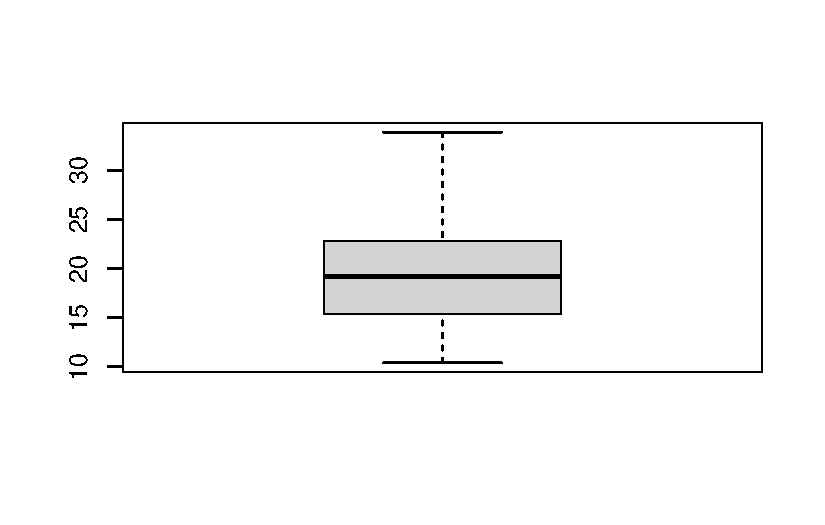
\includegraphics[keepaspectratio]{Descriptive_statistics_in_R_files/figure-pdf/unnamed-chunk-29-1.pdf}}

Same example with \texttt{ggplot} :

\begin{Shaded}
\begin{Highlighting}[]
\NormalTok{mtcars }\SpecialCharTok{|\textgreater{}} 
  \FunctionTok{ggplot}\NormalTok{(}\FunctionTok{aes}\NormalTok{(}\AttributeTok{y =}\NormalTok{ mpg)) }\SpecialCharTok{+}
  \FunctionTok{geom\_boxplot}\NormalTok{()}
\end{Highlighting}
\end{Shaded}

\pandocbounded{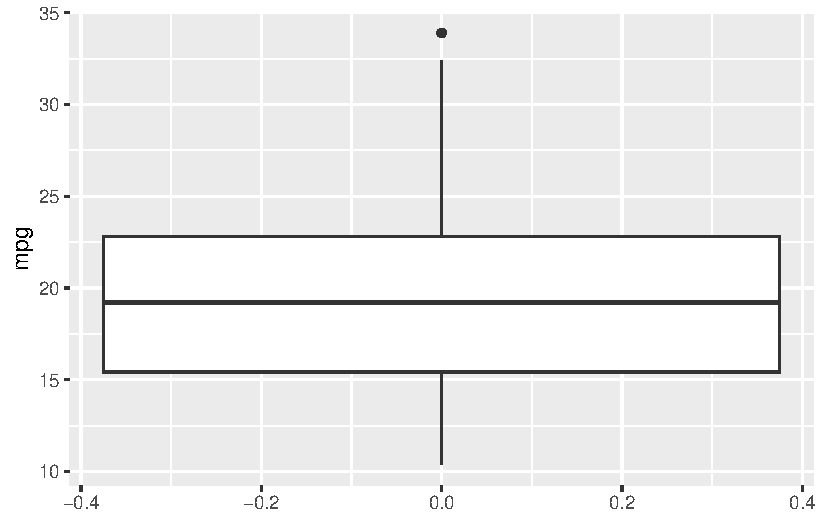
\includegraphics[keepaspectratio]{Descriptive_statistics_in_R_files/figure-pdf/unnamed-chunk-30-1.pdf}}

Note that we omitted the first argument in \texttt{ggplot} given that we
are using a pipe, \texttt{\textbar{}\textgreater{}}. Using pipes is very
handy, since it's easier to see the flow of the computations this way.
We will explain pipes and their use later in the course.




\end{document}
